\documentclass[10pt,twocolumn,letterpaper]{article}

\usepackage{cvpr}
\usepackage{times}
\usepackage{epsfig}
\usepackage{graphicx}
\usepackage{amsmath}
\usepackage{amssymb}

%%%%%%%%%%%%%%
% Packages and stuff custom
%%%%%%%%%%%%%%
\usepackage{url}
\usepackage{amsthm}
\usepackage{color}
\usepackage{subcaption}
\captionsetup{compatibility=false}
\usepackage{booktabs}
%\usepackage{hyperref}
% If you comment hyperref and then uncomment it, you should delete
% egpaper.aux before re-running latex.  (Or just hit 'q' on the first latex
% run, let it finish, and you should be clear).
\usepackage[pagebackref=true,breaklinks=true,letterpaper=true,colorlinks,bookmarks=false]{hyperref}

\DeclareMathOperator{\E}{\mathbb{E}}
\DeclareMathOperator{\R}{\mathbb{R}}

\def\figref#1{Fig.~\ref{#1}}
\def\secref#1{\S\ref{#1}}
\def\tabref#1{Table~\ref{#1}}
\def\eqnref#1{Eq.~\ref{#1}}

\newcommand{\ow}[1]{\textbf{\textcolor[rgb]{.1, .1, .8}{OW: #1}}}
\newcommand{\todo}[1]{\textbf{\textcolor[rgb]{.8, .1, .1}{#1}}}

\DeclareGraphicsExtensions{.pdf,.jpg}

%%%%%%%%%%%%%%%

\graphicspath{ {images/}{syntheticExp/} {final_images/channel_gated/} {final_images/}}
%%%%%%%%%%%%%%%%


% Include other packages here, before hyperref.

% If you comment hyperref and then uncomment it, you should delete
% egpaper.aux before re-running latex.  (Or just hit 'q' on the first latex
% run, let it finish, and you should be clear).
\usepackage[pagebackref=true,breaklinks=true,letterpaper=true,colorlinks,bookmarks=false]{hyperref}

% \cvprfinalcopy % *** Uncomment this line for the final submission

\def\cvprPaperID{****} % *** Enter the CVPR Paper ID here
\def\httilde{\mbox{\tt\raisebox{-.5ex}{\symbol{126}}}}

% Pages are numbered in submission mode, and unnumbered in camera-ready
\ifcvprfinal\pagestyle{empty}\fi
\begin{document}

%%%%%%%%% TITLE
\title{GANGATE}

\author{Arnab Ghosh\\
University of Oxford\\
{\tt\small arnab.ghosh@eng.ox.ac.uk}
% For a paper whose authors are all at the same institution,
% omit the following lines up until the closing ``}''.
% Additional authors and addresses can be added with ``\and'',
% just like the second author.
% To save space, use either the email address or home page, not both
\and
Puneet Dokania\\
University of Oxford\\
{\tt\small puneet@robots.ox.ac.uk}
\and
Richard Zhang\\
Adobe Research\\
{\tt\small rizhang@adobe.com}
\and
Oliver Wang\\
Adobe Research\\
{\tt\small owang@adobe.com}
\and
Philip Torr\\
University of Oxford\\
{\tt\small philip.torr@eng.ox.ac.uk}
\and
Eli Shechtman\\
Adobe Research\\
{\tt\small elishe@adobe.com}
}

%\maketitle
%\thispagestyle{empty}


\twocolumn[{%
\renewcommand\twocolumn[1][]{#1}%
\maketitle
\begin{center}
    \centering
    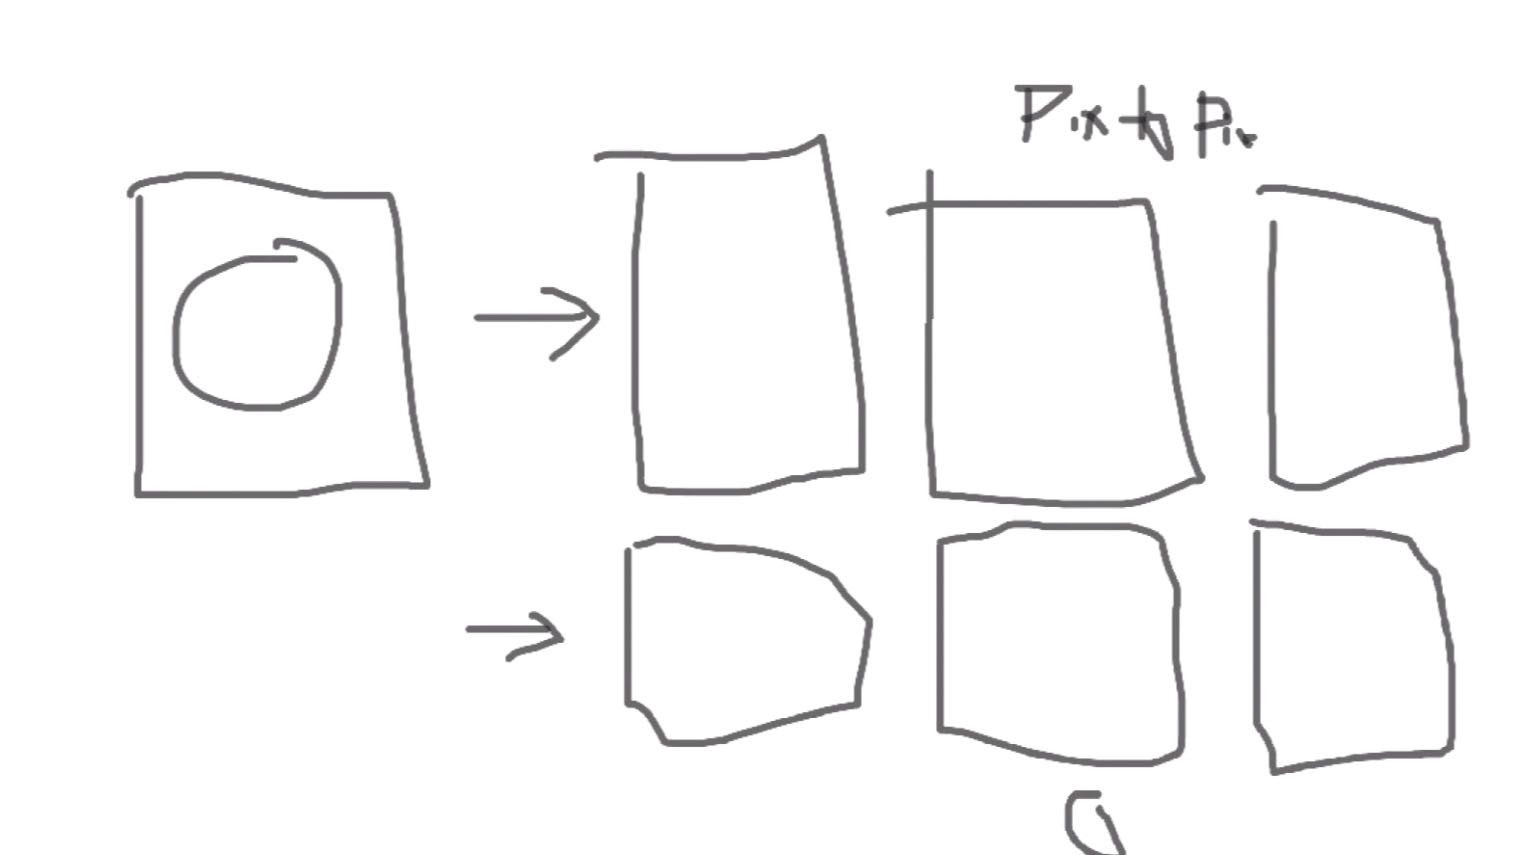
\includegraphics[width=.9\linewidth,height=4.5cm]{images/teaser/sketch.jpg}
    \captionof{figure}{Beautiful teaser with results.}
\end{center}%
}]

%%%%%%%%% ABSTRACT
\begin{abstract}
We propose a method that allows us to generate images belonging to multiple domains using a single network. 
Our approach is based on a GAN framework with two separate branches, a fully residual network, and a separate smaller gating network conditioned on the input class that selects residual blocks from the first branch.
The same gating network also conditions the residual blocks of the discriminator network.
We show that such an approach is able to produce high quality multi-class image generation, both in an image-to-image translation task, as well as a random-noise-to-image generation task. 
This method allows for significantly smaller model sizes than previous multi-class approaches by taking advantage of similarities across classes. 
We analyze our gating network to show that it leads to subnetworks based on the residual blocks that are active for a particular class.
%This approach as well as helps inject low dimensional information into a network more effectively than just concatenating channel-wise after replication to match the image dimension. 
Information theoretic results also show it to be a much stronger form of conditioning than naive concatenation. 
We apply our approach on a novel setting of multi-class outline-to-image generation, where baseline solutions fail to generate good results, while our model successfully tackles the multi-class image generation setting. 
\end{abstract}

\section{Introduction}
Generative methods have made huge strides in the last few years driven by the success of Variational Autoencoders (VAEs)~\cite{kingma2013auto} and Generative Adversarial Networks (GANs)~\cite{goodfellow2014generative}. 
While these methods can generate impressive results, one major challenge is that quality degrades quickly when the diversity of training data increases, especially when the manifold of the multi-class distribution of images drawn from the ground truth distribution is not continuous. \ow{um... I don't really get this previous sentence}

We propose a solution to generate multi-class images using a form of class conditioning that outperforms prior class conditioned GANs while requiring significantly fewer parameters than using a single GAN per-class. 
To do this, we take advantage of the fact that different classes will share similar visual features, and propose an architecture that learns to pick a subset of parameters to use for each class.
Our method leverages a fully-residual GAN architecture, both in the generator and discriminator. 
The fully residual nature allows a second, ``gating'' network to determine which set of generator and discriminator blocks to use conditioned on the input class. \ow{explanation gets harder if ``our'' method is channel-wise}

This gating network serves to perform a form of class conditioning, and we compare the effect of it to a number of other forms of conditioning, such as for example concatenating one-hot class information, auxillary classification, \todo{...}.
\ow{describe high level idea and outcome of the 1d experiments}

We evaluate our gating approach on a number of applications \todo{...}
\ow{discuss evaluation and findings}

In summary, our Contributions are :
\begin{itemize}
\item Incision experiments on a trained Residual Generator based GAN on the 1D Mixture of Gaussians to show certain blocks correspond to certain modes in the generated distribution.
\item Introduction of the Gated Residual Blocks and the Hypernetwork to predict the corresponding alphas on the Generator and Discriminator.
\item Introduction of a new task based on Generative Adversarial Networks namely the task of generating high resolution realistic images from very rough and sparse outline like scribbles.
\end{itemize}

\section{Related Work}
The seminal work by \cite{miyato2018spectral}, introduced spectral normalization which normalizes the weights of the network such that the maximum eigen value of the resulting set of weights is bounded. It helped enormously in stabilizing the training of GANs and albeit they only applied spectral normalization to the discriminator, SA-GAN \cite{zhang2018self} applied it to both the generator and discriminator and showed superior generative modeling performance over several tasks. SA-GAN further introduced the self attention layer based on the innovative transformer network and showed not only better geometric properties being modeled by the GAN but also allowing Multi-Class generations. The Projection Discriminator \cite{miyato2018cgans} based Conditional GANs altered the naive model of concatenating the condition provided to the discriminator via a generalized bilinear projection between the condition and the features extracted from the image thereby providing more finegrained gradients suitable for training the generator to produce class conditional and better resolution images. MAD-GAN \cite{ghosh2017multi} introduced multiple generators and showed an innovative experiment whereby they mixed images from 3 classes and the 3 generators could disentangle the classes and each of the generators generated much sharper images from a particular class than a single generator with similar capacity could. 

%moved from intro
To combat this challenge a solution called MAD-GAN \cite{ghosh2017multi} was proposed which dealt with the issue via multiple generators whereby the discriminator distributed the modes and classes in the data distribution among the various generators. 
Although MAD-GAN was a novel solution to deal with discontinuities in the manifold of the multi-class data distribution, the solution came with its flaws, supreme among them was the reduced scalability in the case the structure was not shared among the different classes, the generators couldn't share the initial layers' parameters and therefore was limited by GPU capacity and in practice going more than 5-6 generators was difficult. 

In another line of papers which helped build the ideas in this paper are the research on Residual Networks \cite{he2016deep} which introduced a set of architectures which allowed extremely deep networks to be trained upto hundreds of layers which was earlier assumed to be extremely difficult because of the problem of vanishing gradients in deep networks. The residual connection allowed a unadulterated gradient backpropagation pathway which enabled training of ultra deep networks. A thorough analysis of residual networks by \cite{liao2016bridging} showed that residual networks have similar connections to unrolled recurrent neural networks without weight sharing and is very similar to how computation unfolds in human brains. Veit et al. \cite{veit2016residual} did a set of innovative incision experiments whereby they removed some blocks and allowed only the skip connection to be active in a trained Residual Network and they were able to demonstrate that even after removing some layers there a very miniscule reduction in the classification accuracy while a similar incision in a VGG network \cite{simonyan2014very} which doesn't have skip connections led to almost random outputs in the task of classification. \cite{veit2016residual} also demonstrated that residual networks behave as an ensemble of several shallower networks. \cite{veit2018adaptive} used the concepts introduced in \cite{veit2016residual} to introduce a discrete gating mechanism in deep residual networks based on the Gumbel-Softmax approximation to make the discrete decision differentiable. Their approach allowed redundant computations in the residual blocks to be reduced and to use only few of the blocks in the trained network during testing phase of the neural network. \cite{de2017modulating} introduced a technique for modulating the activations of a residual block by predicting the parameters of batch normalization which they term as Conditional Batch Normalization. In a similar vein \cite{perez2017film} also used a similar technique for modulating the activations of the various blocks conditioned on the question in a Visual Question Answering scenario.

Gating mechanisms have generally been useful for language modeling tasks such as LSTMs \cite{Hochreiter1997LSTM} and \cite{chung2014empirical} which improved language modeling performance over vanilla RNNs. Gating also helped in the case of image recognition as demonstrated in Highway Networks \cite{srivastava2015highway} albeit it has a lot of resemblance to residual networks. 

Image manipulation and Generation has seen huge strides in recent years with the advent of Generative Adversarial Networks \cite{goodfellow2014generative}, style transfer networks \cite{gatys2015neural} and image colorization \cite{zhang2016colorful}. iGAN \cite{zhu2016generative} was one of the first very innovative papers that introduced us to a novel technique for editing images using neural networks and preventing the edited images to fall off the natural image manifold. Pix2pix \cite{isola2016image2image} introduced a novel network based on GANs which could translate images on a plethora of datasets such as edges to handbags, semantic layout to photo realistic images and day to night. Cutting edge techniques on similar lines include \cite{wang2018video} which can translate from Video to Video such as from pose sequences to a person dancing or from semantic layouts to photorealistic road scenes. InfoGAN \cite{chen2016infogan} introduced a novel network based on GANs and Information Theoretic principles which could disentangle modes in the data distribution based on an unsupervised objective but showed poor performance in being able to disentangle modes and produce stochastic variations in the setting of pix2pix which is known to collapse to a single output for a particular input whereas ideally it should be a distribution. Bicycle GAN \cite{zhu2017toward} introduced 2 cycles which was able to produce stochastic generated outputs in the case of image to image translation. Another innovation was CycleGAN \cite{zhu2017unpaired} which allowed unpaired image to image translation as well as unpaired domain transfer which enabled several transformations which wasn't possible earlier. 

\newcommand{\addSubFigHalf}[3]{\begin{subfigure}[t]{.45\linewidth}
   \includegraphics[width=\linewidth]{#1}
   \caption{#2}\label{#3}\end{subfigure}
}

\begin{figure}[t]
    \centering
    \addSubFigHalf{Picture33.png}{Generated Samples from the trained Generator}{fig:1d_gen} 
    \addSubFigHalf{Picture3.png}{Generated Samples from the trained Generator with one of the blocks removed}{fig:1d_gen_rem} 
    \caption{Generations in MoG 1D setting}
    \label{fig:infogan_bags}
    \vspace{-3mm}
\end{figure}


\section{Preliminaries}

\subsection{\ow{these are from intro}}

\ow{moved, we don't want to make us just look like veit++}
There was an interesting set of experiments performed in \cite{veit2016residual} which showed that residual networks behaved as an ensemble of several shallower networks.
In one interesting experiment  some of the residual blocks were removed out of a trained network and the incised network was still able to perform almost as well inspite of several of these residual blocks being bypassed. 
The above principles led us to a model based on a soft gating mechanism whereby a hypernetwork gets the condition modulates the feature activations of the residual blocks i.e. the output of the standard residual block was modified from $x+f(x)$ to  $x+\alpha . f(x)$ where the set of alphas for each of the residual block is predicted by the hypernetwork. 


Our experiments with the gate selection block on the quintessential MNIST dataset show its efficacy in a limited setting, we further show that infogan based network could be applied to the pix2pix experiments which was earlier known to produce the delta distribution and only a single plausible output \cite{ghosh2017multi}. The resulting infogan based network was able to produce stochastic variations on the generated samples for the task of edges to handbags. We further show the efficacy of the model in the case when we have explicit class information and use it for a novel task of multi-class scribble to image generation. 

We show an interesting set of experiments in the 1D setting of Mixture of Gaussians as was performed in \cite{ghosh2017multi}. A model was trained with the generator composed of residual blocks and then in line with the experiments performed in \cite{veit2016residual} we removed certain residual blocks and allowed the information to flow through the skip connection and we found that removal of certain modes corresponded to the removal of certain residual blocks hence supporting the arguments in \cite{veit2016residual} that residual networks behave as an ensemble of several shallower networks even in the case of generative models.





\subsection*{GANs:} 


\begin{align}\label{eq:ganObjective}
     \min_{\theta_g}\max_{\theta_d}\; & V(\theta_d, \theta_g) := \E_{x \sim p_{d}} \log D(x; \theta_d) \nonumber \\&
     + \E_{z \sim p_z } \log \big( 1 - D(G(z; \theta_g) ; \theta_d)\big) 
\end{align}



Here we present a brief review of GANs~\cite{goodfellow2014generative}. Given a set of samples $\mathcal{D} = (x_i)_{i=1}^n$ from the true data distribution $p_d$, the GAN learning problem is to obtain the optimal parameters $\theta_g$ of a generator $G(z;\theta_g)$ that can sample from an approximate data distribution $p_g$, where $z \sim p_z$ is the prior input noise (\eg samples from a normal distribution). In order to learn the optimal $\theta_g$, the GAN objective (Eq. \eqref{eq:ganObjective}) employs a discriminator $D(x; \theta_d)$ that learns to differentiate between a {\em real} (from $p_d$) and a {\em fake} (from $p_g$) sample $x$. The overall GAN objective is:


The above objective is optimized in a block-wise manner where $\theta_d$ and $\theta_g$ are optimized one at a time while fixing the other. For a given sample $x$ (either from $p_d$ or $p_g$) and the parameter $\theta_d$, the function $D(x; \theta_d) \in [0, 1]$ produces a score that represents the probability of $x$ belonging to the true data distribution $p_d$ (or probability of it being real). The objective of the discriminator is to learn parameters $\theta_d$ that maximizes this score for the true samples (from $p_d$) while minimizing it for the fake ones $\tilde{x} = D(z; \theta_g)$ (from $p_g$). In the case of generator, the objective is to minimize $\E_{z \sim p_z}\log \big( 1 - D(G(z; \theta_g) ; \theta_d) \big)$, equivalently maximize $\E_{z \sim p_z} \log D(G(z; \theta_g) ; \theta_d)$. Thus, the generator learns to maximize the scores for the fake samples (from $p_g$), which is exactly the opposite to what discriminator is trying to achieve. In this manner, the generator and the discriminator are involved in a minimax game where the task of the generator is to maximize the mistakes of the discriminator. Theoretically, at equilibrium, the generator learns to generate real samples, which means $p_g = p_d$.

\subsection*{Residual Networks:}
There was the standard degradation problem in deep neural networks that even after adding more layers to a network the performance of the network doesn't increase . Residual Networks\cite{he2016deep} address the degradation problem by introducing a deep residual learning framework. Instead of hoping each few stacked layers directly fit a desired underlying mapping, they explicitly let these layers fit a residual mapping. Formally, denoting the desired underlying mapping as H(x), they let the stacked nonlinear layers fit another mapping of $F(x):=H(x)-x$. The original mapping is recast into $F(x)+x$. The hypothesis is that it is easier to optimize the residual mapping than to optimize the original mapping. To the extreme, if an identity mapping were optimal, it would be easier to push the residual to zero than to fit an identity mapping by a stack of nonlinear layers.



\subsection*{Generative Network Incision:}
We began with some experiments on a 1D scenario of 1D Mixture of Gaussians, since GANs are generative models, it is apt that we first understand the effect of residual blocks on the Generator of a GAN first in a simple scenario. We first trained a generator and discriminator pair built entirely of residual blocks on the simple setting of 1D distribution. Subsequently on a similar vein as in \cite{veit2016residual} some incision experiments were performed to analyze the performance of the various residual blocks in this setting. An interesting observation was that when some residual blocks were disabled and only the skip connection of that block was activated it led to the disappearance of particular modes from the data distribution. Removal of groups of blocks led to the disappearance of clusters of modes from the generated distribution. This experiment laid the foundation for our Gated Residual Blocks.

\begin{figure*}%[ht!]
    \centering
    \addSubFigHalf{Picture13.png}{Gated Residual Blocks for the Generator}{fig:gru_gen} 
    \addSubFigHalf{Picture14.png}{Gated Residual Blocks for the Discriminator}{fig:gru_dis} 
    \caption{Gated Residual Blocks in Generator and Discriminator}
    \label{fig:model}
    \vspace{-3mm}
\end{figure*}

\section{Gated Residual Block based Generator}
Inspired by the incision experiments performed on the generator whereby removal of certain blocks led to the removal of particular modes from the data distribution, our model consists of a main network which is oblivious to the condition provided to the network, while another hypernetwork only receives the condition and has to predict which block should be used to what extent. More precisely, the $i^{th}$ residual block now receives an extra input $\alpha_i$ alongside the usual $x$ and the output of the gated residual block is $x+\alpha_i*f_i(x)$ rather than the standard $x+f_i(x)$. The $alpha_i$s are predicted via another hypernetwork which only receives the condition and has no idea about the input being received by the main block. The interpretation of the above is that if some block doesn't have to be used for a particular class then the hypernetwork can just choose the $alpha_i$ close to 0 and effectively that block is switched off. The intuition is that the hypernetwork has to first understand the transformations that the different residual blocks in the generator are learning, then start modulating it such that conditioned on the class the required blocks are chosen to the right extent such that the resulting sequence of transformations corresponds to realistic images from that particular class. Its related to FILM \cite{perez2017film} albeit it does feature wise transform and has to predict more parameters than a single number per block. \figref{fig:gru_gen} illustrates the concept in the setting of the conditional generator. Some other extensions such as affine gating per residual block and channel wise gating with its affine counterpart exists as well apart from the well known Adaptive Instance Normalization \cite{huang2017arbitrary} . The varied forms of gating could be applied to the Infogan setup with the gate prediction block receives the randomly sampled latent as input to decide the gates on the various blocks while the Q network trying to reconstruct back the latent that was passed.
 
\section{Gated Residual Block based Discriminator}

Based on a similar principle as the Generator, the Discriminator can also be equipped with gated residual blocks whereby each residual block would compute $x+\alpha_i*f_i(x)$ in place of the standard $x+f_i(x)$ where each $alpha_i$ is predicted by another hypernetwork which gets the condition that which class is the network currently judging for real/fake. Its intriguing that with just the class information the hypernetwork is able to select blocks which effectively guide the discriminator to judge whether its real/fake conditioned on the class. Via accurate gradients backpropagated to the generator it also enables the generator to generate class conditioned high resolution image samples. Intuitively, the discriminator distributes some common functions between the different classes to some of these shared residual blocks which are activated for all classes while the rest of the transformations it distributes in a non-overlapping manner to some specific residual blocks of the discriminator network. Such a concept can not only be used for the discriminator but in many settings where the conditioning variable is known, for example some plausible applications can be the Q network in InfoGAN\cite{chen2016infogan} or the Conditional Inference Network in a CVAE \cite{sohn2015learning}. \figref{fig:gru_dis} illustrates the concept in the setting of the conditional discriminator. Some other extensions such as affine gating per residual block and channel wise gating with its affine counterpart exists as well apart from Adaptive Instance Normalization(AdaIN) \cite{huang2017arbitrary}



\section{Experiments}
We present the details of a set of experiments performed and the corresponding results of the experiments which show the efficacy of our Gated Residual Blocks albeit being simple to implement.

\subsection{Non Parametric Density Estimation:}
\begin{figure}
    \centering
    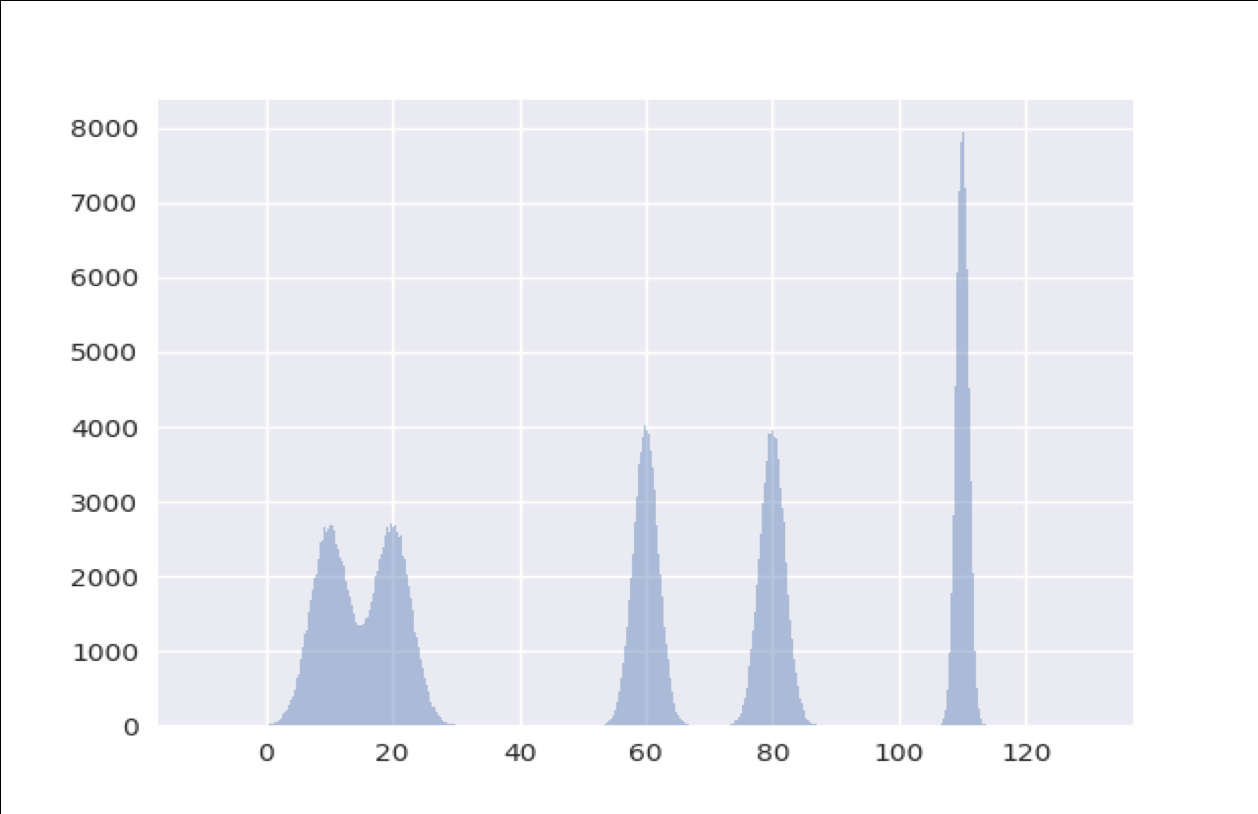
\includegraphics[width=\linewidth]{Picture2}
    \caption{Ground Truth Distribution }\label{fig:1d_ground}
    \vspace{-4mm}
\end{figure}
In order to understand the behavior of the various residual blocks, we first perform a very simple synthetic experiment, much easier than generating high-dimensional complex images. We consider a distribution of 1D Gaussian Mixture \cite{bishop2007pattern} having five mixture components with modes at 10, 20, 60, 80 and 110, and standard deviations of 3, 3, 2, 2 and 1, respectively. While the first two modes overlap significantly, the fifth mode stands isolated as shown in \figref{fig:1d_ground}. We train our resnet block based GAN model using 1 million samples from this distribution and generate 1 million samples from the trained model. In order to compare the learned distribution with the ground truth distributions, we first estimate them using bins over the data points and create the histograms. These histograms are carefully created using different bin sizes and the best bin (found to be 0.1) is chosen. The generated distribution from the trained model corresponds very closely to the ground truth distribution \figref{fig:1d_gen}. The interesting aspect was that although the network was deeper (16 layers of residual blocks) than required for similar experiments in MAD-GAN \cite{ghosh2017multi}, Mode Regularized GAN \cite{che2016mode} and Unrolled GAN \cite{metz2017unrolledGAN}, there were only 4 neurons in each residual block with 16 layers of 4 neurons each in the generator and discriminator compared to fully connected versions in which there consisted of connections between 256 neurons in the preceding layer to 256 neurons in the current layer. Thus although the number of parameters were less, the network learnt the distribution quite accurately.

The next set of experiments was the incision experiments similar to \cite{veit2016residual} on the generator after the network is trained. More specifically, if a layer (say $i^{th}$) had to be skipped, we disable the $f_i(x)$ of the ith residual block and now the output of the $i^{th}$ residual block is $x$ in place of the usual $x+f_i(x)$ encountered during training. Some interesting observations could be made, for example removing some blocks corresponded to the vanishing of certain modes from the generated distribution once the incision was performed on the generator network. Another surprising observation was that the same mode vanished on the incision of certain different residual blocks. This experiment validated the hypothesis of \cite{veit2016residual} that residual networks behave like an ensemble of several shallower networks and also pointed out that another network could predict based on the condition which blocks to use and to skip other non-necessary blocks in the network for that particular condition.

\paragraph{Architecture}


\begin{table}[ht]
\caption{Resblock} % title of Table
\centering % used for centering table
\begin{tabular}{c} % centered columns (4 columns)
\hline\hline %inserts double horizontal lines
F(x)\\%heading
\hline % inserts single horizontal line
Linear(4,4)\\ % inserting body of the table
ReLU() \\
Linear(4,4) \\
\hline %inserts single line
\end{tabular}
\label{table:resblock} % is used to refer this table in the text
\end{table}


\begin{table}[ht]
\caption{Generator} % title of Table
\centering % used for centering table
\begin{tabular}{c c} % centered columns (4 columns)
\hline\hline %inserts double horizontal lines
layer & num layers\\%heading
\hline % inserts single horizontal line
Linear(10,4) & 1\\ % inserting body of the table
ResBlock & 16 \\
Linear(4,1) & 1 \\
\hline %inserts single line
\end{tabular}
\label{table:1d_G} % is used to refer this table in the text
\end{table}

\begin{table}[ht]
\caption{Discriminator} % title of Table
\centering % used for centering table
\begin{tabular}{c c} % centered columns (4 columns)
\hline\hline %inserts double horizontal lines
layer & num layers\\%heading
\hline % inserts single horizontal line
Linear(1,4) & 1\\ % inserting body of the table
ResBlock & 16 \\
Linear(4,1) & 1 \\
Sigmoid & 1 \\
\hline %inserts single line
\end{tabular}
\label{table:1d_D} % is used to refer this table in the text
\end{table}


\subsection{InfoGAN based Model}
The intuitions gained from the experiments performed for the non-parametric density estimation led to the Gated Residual Block on the Generator of a GAN. InfoGAN \cite{chen2016infogan} presented a perfect setting to apply the Gated Residual Block in the case of the generator. The first set of experiments were on MNIST and Fashion-MNIST with sets of 10 discrete variables (since there were 10 classes in both of the datasets) and 2 continuous variables whose information was tried to be maximized using the Q network. As can be seen in \figref{fig:infogan_unconditional} the network was able to generate realistic images from the different classes and produce meaningful interpolations by varying the continuous variables as shown in the figure. The exact experimental setting was that the hypernetwork responsible for the predictions of the $alpha^i$s which we term as the gate selection network gets the salient variables and has no information about the random noise sampled for the main network(consisting of gated residual blocks), based on the salient variables received the gate selection network predicts the  $alpha^i$s for all the blocks of the network. The main network is oblivious of the conditioning received in the salient variables and has to generate images coherent with the conditioning since the Q-Network tries to reconstruct back the conditioning received in the form of salient variables. 

\begin{figure}%[ht!]
    \centering
    \addSubFigHalf{Picture34}{MNIST}{fig:infogan_mnist} 
    \addSubFigHalf{Picture35}{Fashion-MNIST}{fig:infogan_fashion_mnist} 
    \caption{Gated Residual Block-InfoGAN on MNIST and Fashion MNIST}
    \label{fig:infogan_unconditional}
    \vspace{-3mm}
\end{figure}

A well known problem in image conditional GAN settings is the tendency to produce realistic outputs but not being able to produce meaningful variations in the generated output. It was especially prevalent in the original pix2pix setting \cite{isola2016image2image} and further research enabled variations such as \cite{ghosh2017multi} and \cite{zhu2017toward}. Although as shown in \cite{ghosh2017multi} the naive infoGAN setting couldn't produce meaningful variations in the pix2pix setting, settling rather for very minute variations. Our Gated Residual Blocks could mitigate some of the problems and did produce variations in the challenging task of edges-to-bag generation as has been demonstrated in \figref{fig:infogan_bags}. By varying the continuous variable smooth interpolations could be obtained between colors and textures which was earlier not possible with the infogan based pix2pix setting. Although the variations along the discrete axis was quite minimal and we are still investigating the cause for the same. The experimental setting in this scenario was that the salient variables were only given to the gate selection network and had to predict the $alpha^i$s for the main network which consisted of gated residual blocks and was oblivious of the conditioning provided in the form of salient variables. The Discriminator network was the standard image conditional discriminator network while the Q network in this scenario was modified to take the generated image as well as the edge map to behave as a image conditional Q Network which tries to reconstruct back the salient variables given to the gate selection network. 

\newcommand{\addSubFigEighth}[3]{\begin{subfigure}[t]{.18\linewidth}
   \includegraphics[width=\linewidth]{#1}
   \caption{#2}\label{#3}\end{subfigure}
}
\begin{figure*}%[ht!]
    \centering
    \addSubFigEighth{Picture8}{Sketch}{fig:bag_sketch} 
    \addSubFigEighth{Picture9}{Varition 1}{fig:bag_1} 
    \addSubFigEighth{Picture10}{Varition 2}{fig:bag_2}
    \addSubFigEighth{Picture11}{Varition 3}{fig:bag_3}
    \addSubFigEighth{Picture12}{Varition 4}{fig:bag_4}
    \caption{The variations produced in the sketch to realistic bag task in the infogan with Gated Residual Block setting for the generator }
    \label{fig:infogan_bags}
    \vspace{-3mm}
\end{figure*}

\subsection{Unconditional Generations}
\begin{figure}
    \centering
    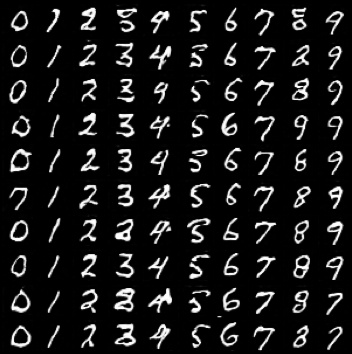
\includegraphics[width=0.5\linewidth]{Picture5}
    \caption{Results on the Gated Residual Block on MNIST dataset}\label{fig:grb_mnist}
    \vspace{-4mm}
\end{figure}

The next set of experiments were performed to judge the robustness of the Gate Selection Blocks and the Gated Residual Blocks in the case the labels were available. That meant using the gate selection network and the gated residual blocks on the discriminator. The implications were even more interesting, the gate selection network would have to distribute the blocks between the classes to get the class specific gradients back for training the class conditioned generator. In the unconditional setting for the generator, the main block only receives random noise and the gate selection block receives the class condition and predicts the $aplha^i$s for the gated residual blocks. The discriminator on the other hand is composed of a main network consisting of gated residual blocks which is oblivious to the class conditioning and a gate selection network which predicts the $aplha^i$s for the main network of the discriminator. The main network predicts how real/fake an image is based on the alpha weightings of its gated residual blocks. The network is able to disentangle the class conditioning although none of the main networks of the generator/ discriminator are aware of the class conditioning, the class information only being input to the gate selection network which has to modulate the weights of the respective networks' gated residual blocks. The generated samples on the MNIST dataset are shown in \figref{fig:grb_mnist} and the alpha gatings for the different classes and the different blocks in \figref{fig:mnist_act}


\begin{figure}%[ht!]
    \centering
    \addSubFigHalf{Picture6}{Activations of the gated residual blocks in the generator}{fig:gen_act} 
    \addSubFigHalf{Picture7}{Activations of the gated residual blocks in the discriminator}{fig:dis_act} 
    \caption{Activation of the various blocks in the Generator and Discriminator}
    \label{fig:mnist_act}
    \vspace{-3mm}
\end{figure}




\subsection{Image Conditional Generations}

\paragraph{Scribble Dataset:}
To test the capability of our techniques on the varied kinds of generation tasks, we collected a dataset of 10 classes with 150 images each from each class. We obtained the scribbles using Adobe Photoshop's tool for outlining objects. We further had a test set consisting of 50 images for each class. The classes collected were basketball,chicken,cookie,cupcake,moon,orange,soccer,strawberry, watermelon, pineapple. 

\newcommand{\addSubFigTenth}[3]{\begin{subfigure}[t]{.16\linewidth}
   \includegraphics[width=\linewidth]{#1}
   \caption{#2}\label{#3}\end{subfigure}
}

\begin{figure*}%[ht!]
    \centering
    \addSubFigTenth{acgan_baseline_all/basketball_11_real_A.png}{}{fig:basketball_scribble} 
    \addSubFigTenth{acgan_baseline_all/chicken_2_real_A.png}{}{fig:chicken_scribble} 
    \addSubFigTenth{acgan_baseline_all/cookie_13_real_A.png}{}{fig:cookie_scribble}
    \addSubFigTenth{acgan_baseline_all/cupcake_27_real_A.png}{}{fig:cupcake_scribble}
    \addSubFigTenth{acgan_baseline_all/moon_15_real_A.png}{}{fig:moon_scribble}
    \addSubFigTenth{acgan_baseline_all/basketball_11_fake_B.png}{}{fig:basketball_img} 
    \addSubFigTenth{acgan_baseline_all/chicken_2_fake_B.png}{}{fig:chicken_img} 
    \addSubFigTenth{acgan_baseline_all/cookie_13_fake_B.png}{}{fig:cookie_img}
    \addSubFigTenth{acgan_baseline_all/cupcake_27_fake_B.png}{}{fig:cupcake_img}
    \addSubFigTenth{acgan_baseline_all/moon_15_fake_B.png}{}{fig:moon_img}
    \addSubFigTenth{acgan_baseline_all/orange_17_real_A.png}{}{fig:orange_scribble} 
    \addSubFigTenth{acgan_baseline_all/pineapple_2_real_A.png}{}{fig:pineapple_scribble} 
    \addSubFigTenth{acgan_baseline_all/soccer_18_real_A.png}{}{fig:soccer_scribble}
    \addSubFigTenth{acgan_baseline_all/strawberry_1_real_A.png}{}{fig:strawberry_scribble}
    \addSubFigTenth{acgan_baseline_all/watermelon_17_real_A.png}{}{fig:watermelon_scribble}
    \addSubFigTenth{acgan_baseline_all/orange_17_fake_B.png}{}{fig:orange_img} 
    \addSubFigTenth{acgan_baseline_all/pineapple_2_fake_B.png}{}{fig:pineapple_img} 
    \addSubFigTenth{acgan_baseline_all/soccer_18_fake_B.png}{}{fig:soccer_img}
    \addSubFigTenth{acgan_baseline_all/strawberry_1_fake_B.png}{}{fig:strawberry_img}
    \addSubFigTenth{acgan_baseline_all/watermelon_17_fake_B.png}{}{fig:watermelon_img}
    \caption{ACGAN baseline with Input Provided to all layers of Generator}
    \label{fig:scribble_pix2pix}
    \vspace{-3mm}
\end{figure*}


\begin{figure*}%[ht!]
    \centering
    \addSubFigTenth{channel_gated/basketball_11_real_A.png}{}{fig:basketball_scribble} 
    \addSubFigTenth{channel_gated/chicken_2_real_A.png}{}{fig:chicken_scribble} 
    \addSubFigTenth{channel_gated/cookie_13_real_A.png}{}{fig:cookie_scribble}
    \addSubFigTenth{channel_gated/cupcake_27_real_A.png}{}{fig:cupcake_scribble}
    \addSubFigTenth{channel_gated/moon_15_real_A.png}{}{fig:moon_scribble}
    \addSubFigTenth{channel_gated/basketball_11_fake_B.png}{}{fig:basketball_img} 
    \addSubFigTenth{channel_gated/chicken_2_fake_B.png}{}{fig:chicken_img} 
    \addSubFigTenth{channel_gated/cookie_13_fake_B.png}{}{fig:cookie_img}
    \addSubFigTenth{channel_gated/cupcake_27_fake_B.png}{}{fig:cupcake_img}
    \addSubFigTenth{channel_gated/moon_15_fake_B.png}{}{fig:moon_img}
    \addSubFigTenth{channel_gated/orange_17_real_A.png}{}{fig:orange_scribble} 
    \addSubFigTenth{channel_gated/pineapple_2_real_A.png}{}{fig:pineapple_scribble} 
    \addSubFigTenth{channel_gated/soccer_18_real_A.png}{}{fig:soccer_scribble}
    \addSubFigTenth{channel_gated/strawberry_1_real_A.png}{}{fig:strawberry_scribble}
    \addSubFigTenth{channel_gated/watermelon_17_real_A.png}{}{fig:watermelon_scribble}
    \addSubFigTenth{channel_gated/orange_17_fake_B.png}{}{fig:orange_img} 
    \addSubFigTenth{channel_gated/pineapple_2_fake_B.png}{}{fig:pineapple_img} 
    \addSubFigTenth{channel_gated/soccer_18_fake_B.png}{}{fig:soccer_img}
    \addSubFigTenth{channel_gated/strawberry_1_fake_B.png}{}{fig:strawberry_img}
    \addSubFigTenth{channel_gated/watermelon_17_fake_B.png}{}{fig:watermelon_img}
    \caption{Gated (Channel/Alpha) Results}
    \label{fig:scribble_pix2pix}
    \vspace{-3mm}
\end{figure*}


\newcommand{\addSubFigSixth}[3]{\begin{subfigure}[t]{.30\linewidth}
   \includegraphics[width=\linewidth]{#1}
   \caption{#2}\label{#3}\end{subfigure}
}
% \begin{figure*}%[ht!]
%     \centering
%     \addSubFigSixth{Picture27}{Pizza On Orange}{fig:bag_sketch} 
%     \addSubFigSixth{Picture28}{Pizza on Pizza}{fig:bag_1} 
%     \addSubFigSixth{Picture29}{Pizza on Orange}{fig:bag_2}
%     \addSubFigSixth{Picture30}{Pizza on Strawberry}{fig:bag_3}
%     \addSubFigSixth{Picture31}{Strawberry on Orange}{fig:bag_4}
%     \addSubFigSixth{Picture32}{Orange on Orange}{fig:bag_4}
%     \caption{Pix2pix fails when there are multi-class mappings from similar scribbles to the varying classes}
%     \label{fig:scribble_pix2pix}
%     \vspace{-3mm}
% \end{figure*}

% \begin{figure*}%[ht!]
%     \centering
%     \addSubFigSixth{Picture15}{Pizza 1}{fig:pizza_1} 
%     \addSubFigSixth{Picture16}{Pizza 2}{fig:pizza_2} 
%     \addSubFigSixth{Picture17}{Pizza 3}{fig:pizza_3}
%     \addSubFigSixth{Picture19}{Strawberry 1}{fig:strawberry_1}
%     \addSubFigSixth{Picture20}{Strawberry 2}{fig:strawberry_2}
%     \addSubFigSixth{Picture21}{Strawberry 3}{fig:strawberry 3}
%     \addSubFigSixth{Picture23}{Orange 1}{fig:orange_1}
%     \addSubFigSixth{Picture24}{Orange 2}{fig:orange_2}
%     \addSubFigSixth{Picture25}{Orange 3}{fig:orange_3}
%     \caption{Pix2pix fails when there are multi-class mappings from similar scribbles to the varying classes}
%     \label{fig:scribble_grb}
%     \vspace{-3mm}
% \end{figure*}

In the widely popular image conditioned generative models introduced in Pix2pix by \cite{isola2016image2image} although the results are brilliant, it had the inherent problem of only being applicable to a particular task such as different networks had to be trained for edges to shoes and edges to handbags, although StarGAN \cite{choi2017stargan} mitigated some of the problems but it was only applicable for relatively minute transformations such as changing the characteristics of the face.

To analyze properly the task of multi-class generations in the image conditioned setting we introduce a new task of generating class conditioned realistic images from very rough scribbles. We start off with 3 classes, namely: pizza, strawberry and oranges. A simple pix2pix network fails to identify the different classes and starts injecting weird textures such as pizza on orange or strawberry on pizza as depicted in the results from pix2pix on this task in \figref{fig:scribble_pix2pix}. 

In the conditional setting for the generator, the main block only receives the input scribble and the gate selection block receives the class condition and predicts the $aplha^i$s for the gated residual blocks. The discriminator on the other hand is composed of a main network consisting of gated residual blocks which is oblivious to the class conditioning and a gate selection network which predicts the $aplha^i$s for the main network of the discriminator. The main network also receives the input scribble alongside the generated/real image to predict how real/fake an image is based on the alpha weightings of its gated residual blocks. The network is able to disentangle the class conditioning although none of the main networks of the generator/ discriminator are aware of the class conditioning, the class information only being input to the gate selection network which has to modulate the weights of the respective networks' gated residual blocks. The results of the model are depicted in \figref{fig:scribble_grb} whereby we can clearly see that the network has been able to disentangle the class conditioning and generate textures appropriate for the right class.

\begin{table}[ht]
\caption{ConvResblock} % title of Table
\centering % used for centering table
\begin{tabular}{c} % centered columns (4 columns)
\hline\hline %inserts double horizontal lines
F(x)\\%heading
\hline
Conv2d(nfilters,kernel=3,stride=1,padding=1) \\
InstanceNorm2d(nfilters)\\ % inserting body of the table
ReLU() \\
Conv2d(nfilters,kernel=3,stride=1,padding=1) \\
InstanceNorm2d(nfilters)\\ % inserting body of the table
ReLU() \\
\hline %inserts single line
\end{tabular}
\label{table:convresblock} % is used to refer this table in the text
\end{table}


\begin{table}[ht]
\caption{UpConvResblock} % title of Table
\centering % used for centering table
\begin{tabular}{c} % centered columns (4 columns)
\hline\hline %inserts double horizontal lines
F(x)\\%heading
\hline
Upsample (Nearest Neighbor) \\
ReflectionPad2d(1) \\
Conv2d(nfilters,kernel=3,stride=1,padding=0) \\
InstanceNorm2d(nfilters)\\ % inserting body of the table
ReLU() \\
Conv2d(nfilters,kernel=3,stride=1,padding=1) \\
InstanceNorm2d(nfilters)\\ % inserting body of the table
ReLU() \\
\hline %inserts single line
Shortcut\\
\hline 
Upsample (Nearest Neighbor) \\
ReflectionPad2d(1)\\
Conv2d(nfilters,kernel=3,stride=1,padding=0) \\
\hline
\end{tabular}
\label{table:upconvresblock} % is used to refer this table in the text
\end{table}

\begin{table}[ht]
\caption{DownConvResblock} % title of Table
\centering % used for centering table
\begin{tabular}{c} % centered columns (4 columns)
\hline\hline %inserts double horizontal lines
F(x)\\%heading
\hline
Avgpool 2d \\
ReflectionPad2d(1) \\
Conv2d(nfilters,kernel=3,stride=1,padding=0) \\
InstanceNorm2d(nfilters)\\ % inserting body of the table
ReLU() \\
Conv2d(nfilters,kernel=3,stride=1,padding=1) \\
InstanceNorm2d(nfilters)\\ % inserting body of the table
ReLU() \\
\hline %inserts single line
Shortcut\\
\hline 
Avgpool 2d \\
ReflectionPad2d(1)\\
Conv2d(nfilters,kernel=3,stride=1,padding=0) \\
\hline
\end{tabular}
\label{table:downconvresblock} % is used to refer this table in the text
\end{table}


\begin{table}[ht]
\caption{Generator} % title of Table
\centering % used for centering table
\begin{tabular}{c c} % centered columns (4 columns)
\hline\hline %inserts double horizontal lines
layer & num layers\\%heading
\hline % inserts single horizontal line
Linear(10,4) & 1\\ % inserting body of the table
ResBlock & 16 \\
Linear(4,1) & 1 \\
\hline %inserts single line
\end{tabular}
\label{table:1d_G} % is used to refer this table in the text
\end{table}


\subsection{Comparison to other forms of conditioning in Resblock :}
Conditional Batch Normalization, FiLM and Adaptive Instance Normalization are the techniques which are the most closely related to our methodology. All of these have the benefit of being applicable even without the presence of residual blocks in the architecture. So an exhaustive comparison with all of these methods along with our form of conditioning on the residual blocks is a valid set of experimentation and has to be done to make the paper complete.


\subsection{Multi-Task Generations: }
Since our network is robust enough to be able to generate images conditioned on class and modulation of which blocks to use, it can further be used to generate images which are different in tasks such as the same network could do both day2night and instance maps to realistic generations of street scenes, efficacy in this dataset would show the efficiency of our method as well as Richard pointed out its a well known task which people accept in which evaluation is also slightly easier.


\begin{figure*}%[ht!]
    \centering
    \addSubFigEighth{channel_gated/cityscapes_95_real_A.png}{}{fig:bag_sketch} 
    \addSubFigEighth{channel_gated/cityscapes_95_fake_B.png}{}{fig:bag_1} 
    \addSubFigEighth{channel_gated/night2day_58_5018_to_5000_real_A.png}{}{fig:bag_2}
    \addSubFigEighth{channel_gated/night2day_58_5018_to_5000_fake_B.png}{}{fig:bag_3}
    \caption{Gated(Channel/Alpha) Multi-Task}
    \label{fig:channel_gated_multi-task}
    \vspace{-3mm}
\end{figure*}

\begin{figure*}%[ht!]
    \centering
    \addSubFigEighth{unet_all/cityscapes_95_real_A.png}{}{fig:bag_sketch} 
    \addSubFigEighth{unet_all/cityscapes_95_fake_B.png}{}{fig:bag_1} 
    \addSubFigEighth{unet_all/night2day_58_5018_to_5000_real_A.png}{}{fig:bag_2}
    \addSubFigEighth{unet_all/night2day_58_5018_to_5000_fake_B.png}{}{fig:bag_3}
    \caption{U-Net (conditioning all layers) Multi-Task}
    \label{fig:channel_gated_multi-task}
    \vspace{-3mm}
\end{figure*}

\begin{figure*}%[ht!]
    \centering
    \addSubFigEighth{our_baseline_all/cityscapes_95_real_A.png}{}{fig:bag_sketch} 
    \addSubFigEighth{our_baseline_all/cityscapes_95_fake_B.png}{}{fig:bag_1} 
    \addSubFigEighth{our_baseline_all/night2day_58_5018_to_5000_real_A.png}{}{fig:bag_2}
    \addSubFigEighth{our_baseline_all/night2day_58_5018_to_5000_fake_B.png}{}{fig:bag_3}
    \caption{Our Architecture (conditioning all layers) Multi-Task}
    \label{fig:channel_gated_multi-task}
    \vspace{-3mm}
\end{figure*}



\section{Planned Set of Experiments:}
\subsection{Unconditional Generations :}
Since the model is not restricted to be applicable only in the image to image setting and is more general than that, if we get the unconditional generations working at least on the places dataset and the faces(it also has got some class labels that can be used for conditioned generation). It will be a good generalization. A bit of engineering might be required to get the architecture working on the unconditional case since the structure of the generator and discriminator would be different from the current generator which takes an image as an input and outputs an image of the same resolution. The discriminator in the case of the current image2image experiments employ a patch based discriminator which has to be modified to work in the unconditional generation setting.




% \subsection{Instance Based Generations: }
% As demonstrated by the early experiments I performed with pix2pixhd that it overfits the dataset and simplification of the same instance map led to garbled generations showed that it was unstable to perturbations. Instance based generations could be possible with our model since we already know which pixels are for which class and we can generate instances of each class separately and then stitch together the various class generations into a final image.


% \section{Directions about novelty of approach:} 

% \subsection{Learning to Learn}
% Learning to learn is becoming an increasingly relevant paradigm for deep learning models as the power of the networks increase and we want less hyper parameter tuning. Our model can be perceived as a system whereby the hypernetwork responsible for predicting the $\alpha_i$ of each block is learning by analyzing the function learnt by each block and thereby distributing the blocks between the various different classes for the generator and the discriminator. We will have to look deeply into the literature to identify the connections with the learning to learn paradigm.

% \subsection{Ensembles of several shallower nets (implicit MAD-GAN)}
% The initial motivation of Eli and Oliver was to extend MAD-GAN with the intuitions gained by Andreas Veit's paper on Residual Blocks acting as ensembles of several shallower networks. The structure of the paper at the moment follows that intuition and the experiments on the 1D Mixture of Gaussians demonstrates that residual blocks indeed behave as ensembles of several shallower networks even in the case of generative models.

% \subsection{Effective way of fusing high dimensional and low dimensional information}
% The techniques proposed in this paper provides a way of effectively fusing high dimensional information in the form of images and low dimensional conditioning in terms of class conditioning or sampled conditioning as in the form of InfoGAN. Further the multi-task application demonstrates the efficacy of the fusing of task information alongside the high dimensional information about images.


\section{Discussion}
Its interesting to observe that with a simple residual block on the non-parametric density estimation task that removal of certain blocks corresponds to the removal of modes in the generated distribution and the incision of different blocks corresponding to the removal of the same mode from the generated distribution shows the validity of the claims in \cite{veit2016residual} which says that residual networks behave as an ensemble of several shallower networks. The results with the Gated Residual Blocks on the Generator on the infoGAN configuration for unconditional setting and the image conditional setting proves the efficacy of the gated residual blocks on the respective tasks. The results of the Gated Residual Blocks on the side of the discriminator shows an intriguing observation that inspite the network being oblivious of the class conditioning, the gate selection network aptly distributed the right blocks for the appropriate classes to disentangle the class conditioning. The Gated Residual Blocks has applications beyond GANs and can be potentially in many conditional scenarios such as text to image synthesis or Conditional Variational Autoencoders. 

\section{Conclusion}
The paper introduced a novel model to disentangle image information and low dimensional information using Gated Residual Blocks which was efficient in generating images in the unconditional setting for infoGAN as well as class and image conditioned setting for the pix2pix variant. The paper also introduced the novel task of class conditional realistic image synthesis from rough scribbles, in which the proposed model performed quite favorably.



{\small
\bibliographystyle{ieee}
\bibliography{src/gatedblocks}
}

\end{document}


